\documentclass{beamer}
\usetheme[sectionpage=none,progressbar=head,numbering=counter]{metropolis}
%\usecolortheme{seagull}
%\setbeamertemplate{page number in head/foot}{}
\setbeamertemplate{bibliography item}{\insertbiblabel}
\usepackage{dirtytalk}
\usepackage{listings}
\usepackage{lmodern}
\usepackage{listings}
\usepackage{mathtools}
\usepackage{graphicx}
\usepackage{caption}
\usepackage{stmaryrd}
\usepackage{tikz}
\usepackage{codeanatomy}
\usepackage{xcolor}
\usepackage{forest}
\usefonttheme[onlymath]{serif}
\graphicspath{{./figs/}}
\newcommand{\frontend}{\emph{frontend}}
\newcommand{\BPG}{BPG}
\newcommand{\BPGs}{BPGs}
\newcommand{\CGS}{CGS}
\newcommand{\CGSs}{CGSs}
\newcommand{\HCP}{HCP}
\newcommand{\HCPs}{HCPs}
\newcommand{\ED}{ED}
\newcommand{\EDs}{EDs}
\newcommand{\CDSS}{CDSS}
\newcommand{\CDSSs}{CDSSs}
\newcommand{\BPGLogic}{knowledge-base}
\newcommand{\K}{\mathbb{K}}
\newcommand{\MediK}{$\text{Medi}\K{}$}
\newcommand{\FSM}{\emph{FSM}}
\newcommand{\FSMs}{\emph{FSMs}}
\newcommand{\Var}{\text{Var}}
\newcommand{\LHS}{\emph{\text{LHS}}}
\newcommand{\RHS}{\emph{\text{RHS}}}
\renewcommand{\phi}{\varphi}
\newcommand{\GUI}{GUI}
\newcommand{\GUIs}{GUIs}
\newcommand{\PME}{PME}
\newcommand{\PMEs}{PMEs}
\newcommand{\CIG}{CIG}
\newcommand{\CIGs}{CIGs}
\newcommand{\EHRs}{EHRs}
\newcommand{\ACLS}{ACLS}
\newcommand{\CPR}{CPR}
\newcommand{\CISs}{CISs}
\newcommand{\RTSs}{RTSs}
\newcommand{\ASMs}{ASMs}
\newcommand{\DSL}{\text{DSL}}
\newcommand{\DSLs}{\text{DSLs}}

% Convenience Commands
\newcommand{\cmark}{\text{\ding{51}}}
\newcommand{\xmark}{\text{\ding{55}}}
\newcommand{\greencheck}{{\color{green}\cmark}}
\newcommand{\redcross}{{\color{red}\xmark}}
\newcommand{\cancelcheck}{\bcancel{\cmark}}
\newcommand{\stress}[1]{\underline{\emph{#1}}}

% Scheduling Commands
\newcommand{\Machine}{\mathcal{M}}
\newcommand{\scheduled}{\textit{scheduled}}
\newcommand{\epoch}{\textit{epoch}}

\definecolor{codegreen}{rgb}{0,0.6,0}
\definecolor{codegray}{rgb}{0.5,0.5,0.5}
\definecolor{codepurple}{rgb}{0.58,0,0.82}
\lstdefinestyle{mediksty}{
  keywordstyle=\color{magenta},
  commentstyle=\color{codepurple},
  basicstyle=\ttfamily\footnotesize
}
\lstdefinelanguage{medik}{
  morekeywords={either, or, machine, interface, vars, state, entry, on, do, goto, receives, ~>, =>},
  morecomment=[l]{//},
  morecomment=[s]{/*}{*/}
}

\lstdefinestyle{ksty}{
  keywordstyle=\color{magenta},
  basicstyle=\ttfamily\footnotesize
}
\lstdefinelanguage{k}{
  morekeywords={rule,configuration,=>,syntax,multiplicity,type},
  morecomment=[l]{//},
  morecomment=[s]{/*}{*/}
}

\bibliographystyle{IEEEtran}
%Information to be included in the title page:
\title{\MediK{}: Towards Safe Guidelines-based Clinical Decision Support}
\date{}
\author{%
\texorpdfstring{
\begin{columns}[onlytextwidth]
\column{0.33\textwidth}
  \textbf{Manasvi Saxena} \\
  \footnotesize{\href{mailto:msaxena2@illinois.edu}{\textbf{msaxena2@illinois.edu}}}
\column{0.33\textwidth}
  Shuang Song \\
  \footnotesize{\href{mailto:shuangs3@illinois.edu}{shuangs3@illinois.edu}}
\column{0.33\textwidth}
  Lui Sha \\
  \footnotesize{\href{mailto:lrs@illinois.edu}{lrs@illinois.edu}}
\end{columns}
}{Authors}}%
\institute[]{University of Ilinois at Urbana Champaign}
\begin{document}
\maketitle
\section{Introduction}
\begin{frame}{Preventable Medical Errors (PMEs)}

  PMEs are characterized by \emph{incorrect intended treatment} or
  \emph{incorrect execution} of \emph{intended treatment}.

  \pause
  Studies estimate that PMEs caused:
  \begin{itemize}
    \item \alert{44,000 - 98,000} deaths in 1997
      \cite{DonaldsonBook00}, and \alert{$>$ 250,000} deaths in 2013 \cite{MakaryBMJ16} in the U.S
      alone.
    \item a financial burden of \alert{19.5 billion} dollars in 2008
      \cite{AndelJHCF12}.
  \end{itemize}
\end{frame}

\begin{frame}{Best Practice Guidelines (BPGs)}

  Evidence-based statements that codify recommended treatment for various
  clinical scenarios.

  \begin{itemize}
    \item Utilize results from latest clinical trials.
    \item Make latest diagnosis and treatment information accessible.
    \item Can \alert{mitigate Preventable Medical Errors (PMEs)}.
  \end{itemize}
\end{frame}

\section{Motivating Example}
\begin{frame}{BPG Example - Pediatric Sepsis}
  \begin{itemize}
    \item Sepsis is caused by an extreme response to an infection.
    \item Prompt screening and management can improve outcomes.
  \end{itemize}
  \pause
  \begin{columns}
    \column{0.55\textwidth}
    \begin{figure}
      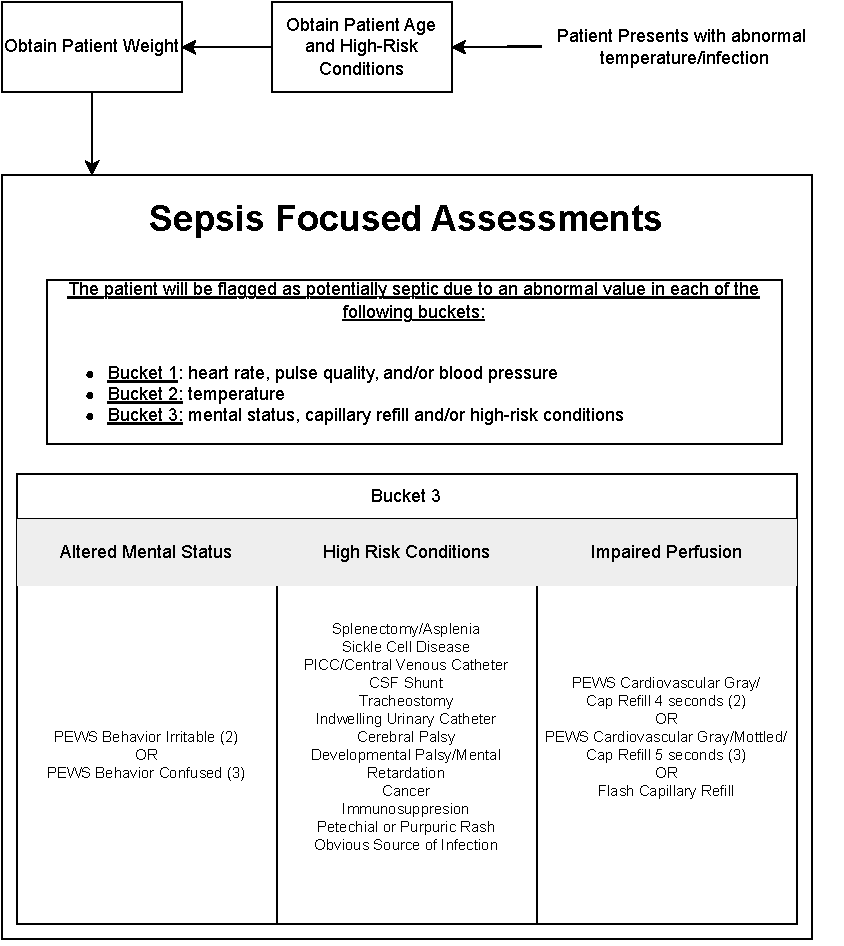
\includegraphics[width=0.8\textwidth]{sepsis-screening-osf}
    \end{figure}
  \column{0.45\textwidth}
    \tiny
    \begin{tabular}{ | c || c | c | }
      \hline
      \textbf{Age}            & \textbf{Heart Rate}    & \textbf{Temp}  \\
      \hline
      $0d - 1m$               & $>205$                 & $<36 \text{ or } >38$ \\
      \hline
      $\geq 1m - 3m$          & $>205$                 & $<36 \text{ or } >38$ \\
      \hline
      $\geq 3m - 1y$          & $>190$                 & $<36 \text{ or } >38.5$ \\
      \hline
      $\dots$                 & $\dots$                & $\dots$ \\
      \hline
      $\geq 13y$              & $>100$                 & $<36 \text{ or } >38.5$ \\
      \hline
    \end{tabular}
  \end{columns}
\end{frame}

%\begin{frame}{Guidelines-based Computerized Decision Support (CDSS)}
%  Systems that codify BPGs to provide healthcare providers with situation-specific advice.
%  \begin{itemize}
%    \item BPG-adherence is difficult to achieve in practice.
%    \item CDSSs integrate BPGs with existing care-flow and make them readily
%      accessible.
%    \item Reduce Preventable Medical Errors \cite{GargJAMA06,KawamotoBMJ05} and improve adherence to BPGs \cite{BenettJAMIA16,SahotaJIS11}.
%  \end{itemize}
%  \pause
%  A typical CDSS consists of:
%  \begin{itemize}
%    \item A translation of the BPG into a computable medium (medical-logic).
%    \item Integration with external data sources such as sensors and electronic
%      records.
%   \item A User-Interface for healthcare providers.
%  \end{itemize}
%\end{frame}

\begin{frame}{Guidelines-based Clinical Decision Support (CDSS)}
  \usetikzlibrary{shapes.geometric, arrows, overlay-beamer-styles}

\tikzstyle{picnode} = [rectangle, minimum size=0.45\textwidth, draw=black]
\tikzstyle{textnode} = [rectangle, rounded corners, text centered, draw=black]

\begin{tikzpicture}[node distance=4cm]

\node (input) [textnode] {
  \tiny
  HCP Assessments
};

\node (cdss) [picnode, right of=input] {
  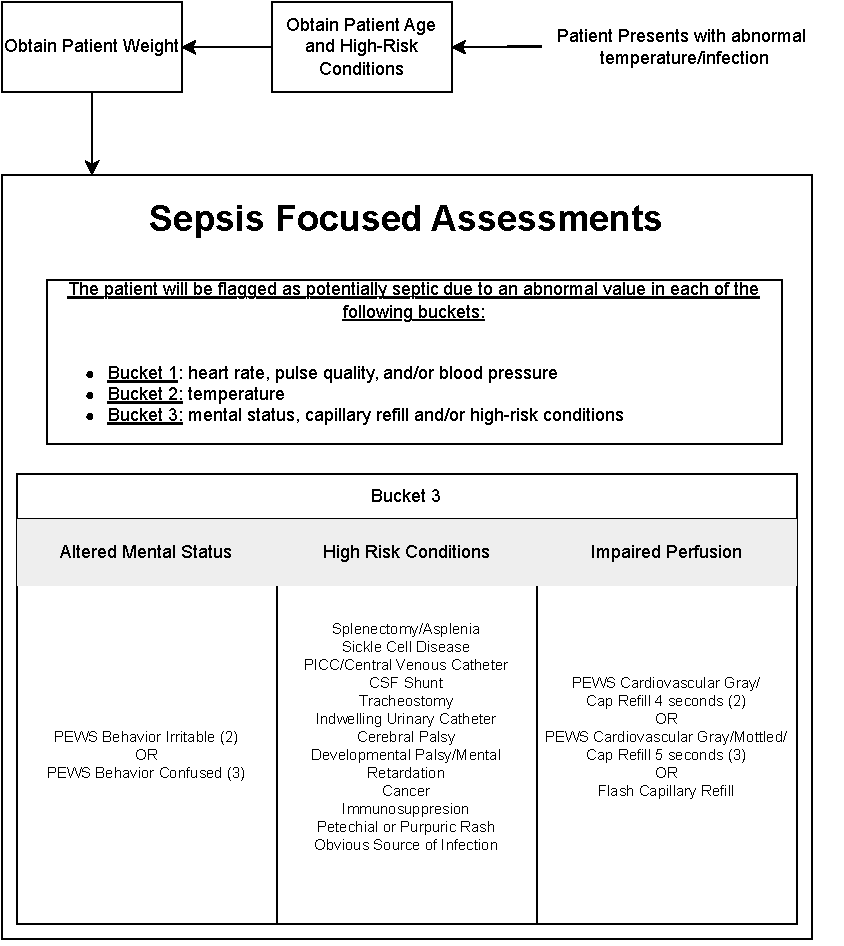
\includegraphics[width=0.4\textwidth]{sepsis-screening-osf}
};

\node (sensor) [textnode, below of=cdss] {
  \tiny
  Sensors + Electronic Health Records
};
\draw<2-> node (advice) [textnode, right of=cdss, fill=red!30] {
  \tiny
  Decision Support
};
\path[->]
  (sensor) edge  (cdss)
  (input) edge (cdss)
  ;

\draw<2-> (cdss) edge[->] (advice);

\end{tikzpicture}

\end{frame}

\begin{frame}{Guidelines-based Clinical Decision Support (CDSS)}
  Broadly, a CDSS will have:
  \begin{itemize}
    \item \textbf{knowledge-base}: BPG translation in a computable medium
    \item \textbf{User Interface}: to enable system interaction
    \item \textbf{Supporting Infrastructure}: to integrate with sensors, patient
      records, and connect components.
  \end{itemize}
  \pause
  Conventionally, to develop a CDSS:
  \begin{itemize}
    \item medical domain experts collaborate with software engineers to
      translate BPG to a programming language
    \item BPG serves as the functional specification
    \item Leads to an \alert{specification-implementation gap}.
  \end{itemize}
\end{frame}

\begin{frame}{Executable Guidelines}
  \begin{itemize}
    \item Both \alert{Comprehensible} to healthcare providers and \alert{executable}
    \item Can directly be used in a CDSS
    \item Address \alert{specification-implementation gap}
      \pause
    \item Existing languages lack complete executable formal semantics,
      and a comprehensive suite of analysis tools.
  \end{itemize}
  \pause
  The \MediK{} language for expressing CDSS knowledge-base:
  \begin{itemize}
    \item Has a complete $\K$-based executable semantics
    \item \emph{Correct-by-construction} tools (including interpreter)
      derived from its semantics
    \item Evolve rapidly to incorporate medical domain experts' feedback

  \end{itemize}
\end{frame}

\begin{frame}{\MediK{}: Executable Guidelines}
  Common characteristics of BPGs:
  \begin{itemize}
    \item \textbf{Concurrent workflows} such as administering
      drugs, performing treatment, monitoring vitals.
    \item \textbf{Flowchart-like notation} for workflows.
    \item \textbf{Heterogeneous agents} such as inputs from sensors, healthcare
      providers.
    \item \textbf{Tables} indexed by parameters like age, weight to indicate
      normal measurement ranges or drug doses.
  \end{itemize}
  \pause
  In \MediK{} guidelines are:
  \begin{itemize}
    \item Expressed as concurrently Finite State Machines (FSMs)
    \item Each flowchart expressed as a FSM
  \end{itemize}
\end{frame}

\begin{frame}[fragile]{Example \MediK{} Guideline}
  \begin{columns}
    \column{0.5\textwidth}
      \begin{tikzpicture}
    \node[anchor=south west,inner sep=0] (cdssimage) at (0,0) {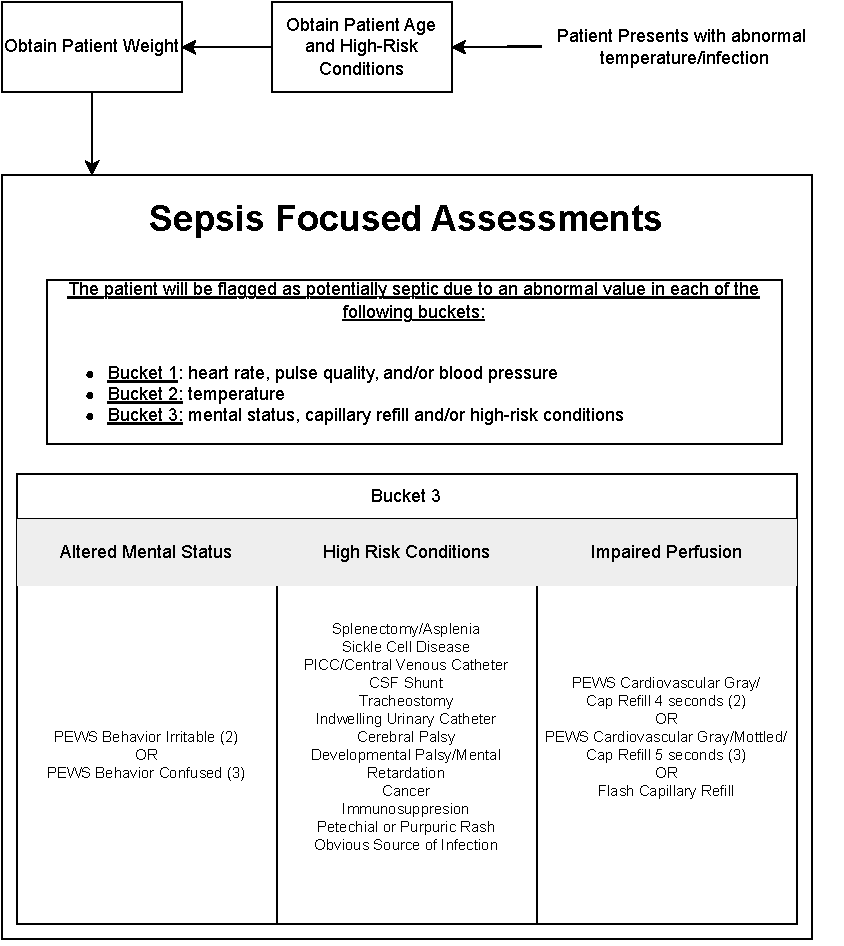
\includegraphics[width=0.9\textwidth]{sepsis-screening-osf}};
    \begin{scope}[x={(cdssimage.south east)},y={(cdssimage.north west)}]
        %\draw[help lines,xstep=.1,ystep=.1] (0,0) grid (1,1);
        %\foreach \x in {0,1,...,9} { \node [anchor=north] at (\x/10,0) {0.\x}; }
        %\foreach \y in {0,1,...,9} { \node [anchor=east] at (0,\y/10) {0.\y}; }
        \draw<2>[red] (0.0001,0.9) rectangle (0.22,0.999);
        \draw<3>[red] (0.0001,0.0) rectangle (0.965,0.82);
    \end{scope}
\end{tikzpicture}

    \column{0.5\textwidth}
    \begin{onlyenv}<2>
      \begin{lstlisting}[language=medik, style=mediksty, basicstyle=\ttfamily\tiny]
state ObtainAge {
  entry {
    send tablet, Instruct, ("get age");
  } on ConfirmAgeEntered do {
    goto ObtainWeight;
  }
}
    \end{lstlisting}
    \end{onlyenv}
    \begin{onlyenv}<3>
      \begin{lstlisting}[language=medik, style=mediksty, basicstyle=\ttfamily\tiny]
state CalculateScore {
  var hrAbnormal = !isInNormalRange(...);
  var bucket1    = hrAbnormal || ...

  var sepsisSuspected
    = bucket1 && bucket2 && bucket3;

  send tablet, SepsisDiagnosis
    , (sepsisSuspected);
}
      \end{lstlisting}
    \end{onlyenv}
  \end{columns}
\end{frame}

\begin{frame}[fragile]{Example \MediK{} Guideline}
  \begin{columns}
  \column{0.33\textwidth}
    \tiny
    \begin{tabular}{ | c || c | c | }
      \hline
      \textbf{Age}            & \textbf{Heart Rate} \\
      \hline
      $0d - 1m$               & $>205$              \\
      \hline
      $\geq 1m - 3m$          & $>205$              \\
      \hline
      $\geq 3m - 1y$          & $>190$              \\
      \hline
      $\dots$                 & $\dots$             \\
      \hline
      $\geq 13y$              & $>100$              \\
      \hline
    \end{tabular}
    \column{0.67\textwidth}
\begin{lstlisting}[
  style=mediksty
  ,language=medik
  ,basicstyle=\ttfamily\tiny
  ]
fun isHeartRateNormal() {
  days(age) in {
    interval(days(0)  , months(1)): return hr > 205;
    interval(months(1), months(3)): return hr > 205;
    // omitting other cases
    default                       : return hr > 100;
  }
}
\end{lstlisting}
  \end{columns}
\end{frame}

\begin{frame}[fragile]{\MediK{}: Formal Semantics}
  %Add a slide on $\K{}$
  \MediK{}'s semantics formalized in the $\K{}$-framework
  \begin{itemize}
    \item All tools (including interpreter) derived from semantics,
      hence \emph{correct-by-construction}
    \item Rapidly incorporate physician feedback - only
      semantics need to be changed. Tools evolve automatically.
  \end{itemize}
  \pause
  The semantics have three components:
  \begin{itemize}
    \item \textbf{Syntax:} Specified
    \item \textbf{Configuration:} Nested \say{cells} that hold execution state
    \item \textbf{Rules:} Transition system over configuration
  \end{itemize}
\end{frame}
\begin{frame}[fragile]{\MediK{} Configuration}

  \lstset {
basicstyle=\tiny\ttfamily
,escapeinside= {!}{!}
}


\begin{overprint}
\begin{tikzpicture}[remember picture, stop jumping, constrain]
  \node (code) [anatomy] at (0,0) {
    \begin{lstlisting}[
      style=ksty
      ,language=k
      ,basicstyle=\ttfamily\scriptsize
      ]
    configuration
     !\mtPoint{mostLeft}! <instance multiplicity="*" type="Map"> ... !\extremPoint{mostRight}!
      !\mtPoint{mostLeftK}!<k> $PGM </k>!\extremPoint{mostRightK}\mbPoint{mostBottomK}!
        <env> .Map </env>
        <inBuffer> .List </inBuffer>
      </instance>!\mbPoint{mostBottom}!
     !\mtPoint{mostLeftMachine}! <machine multiplicity="*" type="Map"> ... !\extremPoint{mostRightMachine}!
        <machineName> . </machineName>
        <states>
          <state multiplicity="*" type="Map">
            <stateName> . </stateName>
            <entryBlock> . </entryBlock>
            <eventHandlers> ... </eventHandlers>
          </state>
        </states>
      </machine>!\mbPoint{mostBottomMachine}!
    \end{lstlisting}
  };
\only<2->{
  \fitExtrem{instanceBox}{(mostLeft) (mostRight) (mostBottom)}
  \codeAnnotation{instanceBoxAnnotation} (10.35,5) {State of \\ running instance} {[on background layer]}
  \draw[->,annotation] (instanceBox) -- (instanceBoxAnnotation);
};
\only<3->{
  \fitExtrem{KBox}{(mostLeftK) (mostRightK) (mostBottomK)}
  \codeAnnotation{KBoxAnnotation} (6.45,5.25) {\MediK{} Program} {[on background layer]}
  \draw[->,annotation] (KBox) -- (KBoxAnnotation);
};

\only<4->{
  \fitExtrem{MachineBox}{(mostLeftMachine) (mostRightMachine) (mostBottomMachine)}
  \codeAnnotation{MachineBoxAnnotation} (10.25,2.3) {Machine \\ Definitions} {[on background layer]}
  \draw[->,annotation] (MachineBox) -- (MachineBoxAnnotation);
};
\end{tikzpicture}
\end{overprint}

\end{frame}
\begin{frame}[fragile]{\MediK{}: Formal Semantics}
  Variable Lookup
  \begin{lstlisting}[language=k,style=ksty,basicstyle=\ttfamily\tiny]
rule <k> I:Id = V:Val => V ... </k>
     <env> (I |-> Loc) ... </env>
     <store> Store => Store[Loc <- V] </store>
  \end{lstlisting}
  \pause
  Sending Events
  \begin{lstlisting}[language=k,style=ksty,basicstyle=\ttfamily\tiny]
rule <instance>
     <k> send instance(RecvId) , EventName:Id , ( Args ) =>  done ... </k>
      ...
    </instance>
    <instance>
     <id> RecvId </id> ....
     <inBuffer> ...
        (.List => ListItem( eventArgsPair(EventName | Args | Epoch + 1)))
     </inBuffer> ...
    </instance>
    <epoch> Epoch </epoch>
  \end{lstlisting}
\end{frame}
\begin{frame}[fragile]{\MediK{}: Model Checking}
  \begin{itemize}
    \item Accomplished by \emph{searching} the transition system for
      an \emph{erroneous} pattern
    \item One important pattern in \MediK{}'s context is \emph{stuck}
    \item Reached when an event does not have an associated handler
  \end{itemize}
  \pause
  \begin{lstlisting}[language=medik,style=mediksty,basicstyle=\ttfamily\tiny]
  rule <k> handleEvents ~> _ => stuck </k>
       <activeState> ActiveState </activeState>
       <class> MachineName </class>
       <inBuffer> ListItem(event(InputEvent | _ | _ )) ... </inBuffer>
       <machine>
        <machineName> MachineName </machineName>
        <state>
         <stateName> ActiveState </stateName>
         <handledEventIds> HandledEvents </handledEventIds> ...
        </state> ...
       </machine>
    requires notBool(InputEvent in HandledEvents)
  \end{lstlisting}
\end{frame}
\begin{frame}{\MediK{}: Model Checking}
  \begin{itemize}
    \item External components treated as Finite State Machines
    \item For model checking, \MediK{} uses \alert{ghost machines}
      to close the system
  \end{itemize}
  Ghost machines additionally support:
  \begin{itemize}
    \item Statements to express \alert{non-determinism}
    \item Abstract encodings for patient parameters
  \end{itemize}
\end{frame}
\begin{frame}[fragile]{\MediK{}: Model Checking}
Abstract Encodings
  \begin{lstlisting}[language=medik,style=mediksty]
on Instruct(instruction) do {
  if (instruction == "get age") {
    broadcast AgeEntered, (#nondet);
    goto Main;
  }
}
\end{lstlisting}
\pause
Non-determinism
\begin{lstlisting}[language=medik,style=mediksty]
either {
  broadcast StartFluidTherapy;
} or {
  broadcast StartAntibioticTherapy;
}
\end{lstlisting}
\end{frame}
\begin{frame}[allowframebreaks]{References}
  \bibliography{references}
\end{frame}
\end{document}
